\documentclass[12pt,a4paper]{article}

\usepackage{iftex}
\ifPDFTeX
  \usepackage[utf8]{inputenc}
  \usepackage[T2A]{fontenc}
\else
  \usepackage{fontspec}
  \setmainfont{cmunrm.otf}[Path=docs/fonts/,BoldFont=cmunbx.otf,ItalicFont=cmunti.otf,BoldItalicFont=cmunbi.otf]
  \setmonofont{cmuntt.otf}[Path=docs/fonts/,BoldFont=cmuntb.otf,ItalicFont=cmunit.otf,BoldItalicFont=cmuntx.otf]
\fi
\usepackage[russian]{babel}
\usepackage{amsmath}
\usepackage{amssymb}
\usepackage{array}
\usepackage{booktabs}
\usepackage{caption}
\usepackage{enumitem}
\usepackage{fancyhdr}
\usepackage{float}
\usepackage{geometry}
\usepackage{graphicx}
\usepackage{hyperref}
\usepackage{indentfirst}
\usepackage{listings}
\usepackage{longtable}
\usepackage{tikz}
\usepackage{xcolor}
\usetikzlibrary{arrows.meta,positioning,shapes.geometric}

\geometry{left=30mm,right=15mm,top=20mm,bottom=20mm}
\setlength{\parindent}{1.25cm}
\linespread{1.2}
\pagestyle{fancy}
\fancyhf{}
\fancyfoot[C]{\thepage}
\renewcommand{\headrulewidth}{0pt}
\hypersetup{hidelinks}

\captionsetup{justification=centering}
\setcounter{tocdepth}{2}

\definecolor{codebg}{RGB}{248,248,248}
\definecolor{codeframe}{RGB}{215,215,215}
\definecolor{codekw}{RGB}{0,76,153}
\definecolor{codestr}{RGB}{163,21,21}
\definecolor{codecomment}{RGB}{0,128,0}
\definecolor{eulercolor}{RGB}{204,112,69}
\definecolor{rkcolor}{RGB}{47,95,167}
\definecolor{adamscolor}{RGB}{124,79,160}
\definecolor{exactcolor}{RGB}{61,124,85}

\lstdefinelanguage{JavaScript}{
  morekeywords={const,let,var,function,return,if,else,for,while,throw,new,export,import,from,class,get,of,in,try,catch,continue,typeof},
  sensitive=true,
  morecomment=[l]{//},
  morestring=[b]",
  morestring=[b]',
}

\lstset{
  language=JavaScript,
  basicstyle=\ttfamily\small,
  keywordstyle=\color{codekw}\bfseries,
  stringstyle=\color{codestr},
  commentstyle=\color{codecomment},
  backgroundcolor=\color{codebg},
  frame=single,
  rulecolor=\color{codeframe},
  numbers=left,
  numberstyle=\tiny,
  stepnumber=1,
  breaklines=true,
  showstringspaces=false,
  tabsize=2,
  columns=fullflexible,
  keepspaces=true,
  extendedchars=true,
  inputencoding=utf8
}

\newcolumntype{C}[1]{>{\centering\arraybackslash}p{#1}}

\begin{document}

% ====================== ТИТУЛЬНЫЙ ЛИСТ ======================
\pagenumbering{gobble}
\hypersetup{pageanchor=false}
\begin{titlepage}
  \thispagestyle{empty}
  \begin{center}
    {\small Федеральное государственное автономное образовательное учреждение высшего образования\\
    «Национальный исследовательский университет ИТМО»}\\[0.8em]
    {\small Факультет программной инженерии и компьютерной техники}

    \vfill

    {\Large\textbf{Лабораторная работа №6}}\\[0.6em]
    {\large «Численное решение обыкновенных\\дифференциальных уравнений»}\\[0.6em]
    {\large по курсу «Вычислительная математика»}\\[0.6em]
    {\large Вариант 19}

    \vfill

    \begin{flushright}
      \begin{tabular}{l}
        Выполнил:\\
        Якименко Владислав Игоревич, Р3213\\[0.8em]
        Проверила:\\
        Малышева Татьяна Алексеевна
      \end{tabular}
    \end{flushright}

    \vfill

    Санкт-Петербург --- 2026
  \end{center}
\end{titlepage}
\clearpage
\hypersetup{pageanchor=true}

\tableofcontents
\thispagestyle{empty}
\clearpage
\pagenumbering{arabic}


% ====================== 1 ======================
\section{Цель работы и постановка задачи}

\textbf{Цель работы:} решить задачу Коши для обыкновенного дифференциального
уравнения первого порядка численными методами, сравнить одношаговые и
многошаговые схемы и оценить погрешность полученных решений.

\subsection{Задача Коши}
Требуется найти функцию $y=y(x)$, удовлетворяющую уравнению первого порядка,
разрешённому относительно производной,
\[
y' = f(x,y),\qquad x\in[x_0,x_n],
\]
и начальному условию
\[
y(x_0)=y_0 .
\]
Решить задачу численно --- значит для последовательности узлов
$x_0<x_1<\dots<x_n$ с постоянным шагом $h=x_{i+1}-x_i$ приближённо вычислить
значения $y_1,\dots,y_n$ сеточной функции, приближающей точное решение
в этих узлах.

Достаточные условия существования и единственности даёт теорема Коши: если
$f(x,y)$ непрерывна в замкнутой области
$\bar D=\{(x,y):|x-x_0|\le a,\;|y-y_0|\le b\}$, решение существует; если,
кроме того, $f$ удовлетворяет условию Липшица по $y$
\[
|f(x,y_1)-f(x,y_2)|\le k|y_1-y_2|,\qquad k=\mathrm{const}>0,
\]
то решение единственно. Геометрически задача Коши --- это поиск интегральной
кривой, проходящей через заданную начальную точку $M_0(x_0,y_0)$.

\subsection{Вариант задания}
Номер варианта --- 19. По таблице 1 задания варианту соответствует набор
методов \textbf{1, 3, 4}:
\begin{itemize}[leftmargin=*]
\item одношаговые: \textbf{метод Эйлера} (метод 1) и
      \textbf{метод Рунге--Кутта 4-го порядка} (метод 3);
\item многошаговый: \textbf{метод Адамса} в схеме предиктор-корректор (метод 4).
\end{itemize}
Точность одношаговых методов оценивается по \textbf{правилу Рунге}, точность
многошагового --- по точному решению: $\varepsilon=\max\limits_{0\le i\le n}
|y_{i\,\text{точн}}-y_i|$.

\subsection{Уравнения, предлагаемые программой}
Задание требует предложить пользователю не менее трёх уравнений. Программа
предлагает шесть; для каждого известно аналитическое решение задачи Коши,
поэтому погрешность можно измерить в каждом узле.

\begin{table}[H]\centering\small
\caption{Уравнения и точные решения задачи Коши}
\begin{tabular}{llp{6.2cm}}\toprule
Идентификатор & $y'=f(x,y)$ & Точное решение\\\midrule
\texttt{linear} & $y$ & $y=y_0e^{x-x_0}$\\
\texttt{sum} & $x+y$ & $y=(y_0+x_0+1)e^{x-x_0}-x-1$\\
\texttt{square} & $y-x^2+1$ & $y=(x+1)^2+Ce^{x}$, $C=(y_0-(x_0+1)^2)e^{-x_0}$\\
\texttt{bernoulli} & $y+(1+x)y^2$ & $y=\dfrac{1}{Ce^{-x}-x}$, $C=e^{x_0}\left(\dfrac{1}{y_0}+x_0\right)$\\
\texttt{gauss} & $-2xy$ & $y=y_0e^{x_0^2-x^2}$\\
\texttt{stiff} & $-5y+5x^2+2x$ & $y=x^2+Ce^{-5x}$, $C=(y_0-x_0^2)e^{5x_0}$\\\bottomrule
\end{tabular}\end{table}

Уравнение \texttt{bernoulli} совпадает с примером 1 лекции: при $y(1)=-1$
постоянная $C=e\left(\tfrac{1}{-1}+1\right)=0$, и точное решение принимает вид
$y=-\dfrac{1}{x}$. Это позволяет сверить работу программы с таблицами,
приведёнными в лекции, поэтому именно эта задача выбрана в качестве основного
демонстрационного набора:
\[
y'=y+(1+x)y^2,\qquad y(1)=-1,\qquad x\in[1;\,1{,}5],\qquad h=0{,}1,\qquad
\varepsilon=10^{-6}.
\]

% ====================== 2 ======================
\section{Описание алгоритма решения задачи}

\subsection{Метод конечных разностей}
Все реализованные методы основаны на методе конечных разностей. Область
непрерывного изменения аргумента --- отрезок $[x_0,x_n]$ --- заменяется
дискретным множеством узлов $x_i=x_0+ih$, образующих разностную сетку.
Искомая функция непрерывного аргумента заменяется сеточной функцией $y_i$,
а дифференциальное уравнение --- разностным уравнением относительно $y_i$;
входящая в уравнение производная заменяется конечно-разностным отношением.
Такая замена называется разностной аппроксимацией на сетке.

\subsection{Общая схема работы программы}
\begin{enumerate}[label=\arabic*.,leftmargin=1.2cm]
\item Пользователь выбирает уравнение $y'=f(x,y)$ из предложенного списка.
\item С клавиатуры (либо из файла) вводятся $x_0$, $y_0=y(x_0)$, правая
граница $x_n$, шаг $h$ и точность $\varepsilon$.
\item Входные данные проверяются: $x_n>x_0$, $h>0$, $h\le x_n-x_0$,
$0<\varepsilon<1$, число узлов не превышает предела, правая часть определена
в начальной точке.
\item Строится сетка $x_i=x_0+ih$, $i=0,\dots,n$; вычисляется точное решение
$y_{i\,\text{точн}}$ в узлах.
\item Задача решается тремя методами варианта. Метод Адамса перед началом
счёта получает $y_1,y_2,y_3$ методом Рунге--Кутта.
\item Составляется общая таблица приближённых значений и погрешностей.
\item Для одношаговых методов выполняется контроль точности по правилу Рунге:
задача решается с шагами $h$ и $h/2$, вычисляется $R$; пока $R>\varepsilon$,
шаг делится пополам.
\item Для метода Адамса вычисляется
$\varepsilon=\max\limits_{0\le i\le n}|y_{i\,\text{точн}}-y_i|$.
\item Строятся графики точного и приближённых решений (разными цветами) и
график погрешности; результаты выводятся в консоль, в файл и в браузер.
\end{enumerate}

\begin{figure}[H]\centering
\begin{tikzpicture}[
  node distance=7mm and 10mm,
  every node/.style={font=\small},
  block/.style={rectangle,draw,rounded corners=2pt,align=center,inner sep=4pt,text width=6.4cm},
  io/.style={trapezium,trapezium left angle=70,trapezium right angle=110,draw,align=center,inner sep=3pt,text width=5.4cm},
  test/.style={diamond,aspect=2.6,draw,align=center,inner sep=1pt,text width=4.6cm},
  line/.style={-{Latex[length=2mm]}}]
\node[io] (in) {Выбор уравнения; ввод $x_0,y_0,x_n,h,\varepsilon$};
\node[block,below=of in] (check) {Проверка данных; сетка $x_i=x_0+ih$; точное решение $y_{i\,\text{точн}}$};
\node[block,below=of check] (one) {Эйлер и Рунге--Кутта: расчёт $y_i$ с шагом $h$ и с шагом $h/2$};
\node[test,below=of one] (runge) {$R=\dfrac{|y_h-y_{h/2}|}{2^p-1}\le\varepsilon$?};
\node[block,below=of runge] (adams) {Адамс: разгон Рунге--Кутта ($y_1,y_2,y_3$), затем предиктор и корректор до $|y^{(k+1)}-y^{(k)}|\le\varepsilon$};
\node[io,below=of adams] (out) {Таблица значений, оценки погрешности, графики};
\draw[line] (in) -- (check);
\draw[line] (check) -- (one);
\draw[line] (one) -- (runge);
\draw[line] (runge) -- node[right,pos=0.4]{да} (adams);
\draw[line] (adams) -- (out);
\draw[line] (runge.east) -- ++(1.6,0) node[above,pos=0.55]{нет: $h\leftarrow h/2$} |- (one.east);
\end{tikzpicture}
\caption{Блок-схема алгоритма программы}
\end{figure}

% ====================== 3 ======================
\section{Рабочие формулы используемых методов}

\subsection{Метод Эйлера (метод 1)}
Метод основан на разложении решения в ряд Тейлора в окрестности узла $x_i$
с отбрасыванием членов, содержащих производные второго и более высоких
порядков:
\[
Y(x_i+h)=Y(x_i)+Y'(x_i)h+O(h^2),\qquad
Y'(x_i)=f(x_i,y_i)\approx\frac{y_{i+1}-y_i}{h}.
\]
Отсюда получается расчётная формула
\begin{equation}
y_{i+1}=y_i+hf(x_i,y_i),\qquad i=0,1,\dots,n-1,
\end{equation}
\begin{equation}
y_0=Y_0 .
\end{equation}
Геометрически на каждом шаге приращение решения заменяется приращением
ординаты касательной, поэтому после первого шага счёт продолжается уже по
другой интегральной кривой. Метод одношаговый, порядок точности $p=1$,
суммарная погрешность $\delta_n=O(h)$.

\subsection{Метод Рунге--Кутта 4-го порядка (метод 3)}
Идея методов Рунге--Кутта: не использовать частные производные $f(x,y)$,
а вычислять саму правую часть в нескольких точках внутри шага. Для наиболее
распространённого метода 4-го порядка:
\begin{equation}
y_{i+1}=y_i+\frac{1}{6}\left(k_1+2k_2+2k_3+k_4\right),
\end{equation}
\begin{equation}
\begin{aligned}
k_1&=h\,f(x_i,\,y_i), &
k_2&=h\,f\!\left(x_i+\tfrac{h}{2},\;y_i+\tfrac{k_1}{2}\right),\\
k_3&=h\,f\!\left(x_i+\tfrac{h}{2},\;y_i+\tfrac{k_2}{2}\right), &
k_4&=h\,f\!\left(x_i+h,\;y_i+k_3\right).
\end{aligned}
\end{equation}
Метод требует четырёхкратного вычисления правой части на каждом шаге,
но имеет суммарную погрешность $\delta_n=O(h^4)$, что позволяет считать
с существенно большим шагом, чем метод Эйлера. Метод одношаговый: значение
$y_{i+1}$ строится только по $y_i$, поэтому шаг можно менять в любой момент.

\subsection{Метод Адамса, схема предиктор-корректор (метод 4)}
Многошаговые методы получаются интегрированием уравнения на отрезке
$[x_i,x_{i+1}]$ с заменой правой части интерполяционным многочленом
$P_{k-1}$, построенным по значениям $f_{i-k+1},\dots,f_i$:
\[
y_{i+1}=y_i+\int\limits_{x_i}^{x_{i+1}}P_{k-1}(x)\,dx .
\]
При $k=4$ и постоянном шаге многочлен Ньютона строится по конечным разностям
правой части
\[
\Delta f_i=f_i-f_{i-1},\quad
\Delta^2f_i=f_i-2f_{i-1}+f_{i-2},\quad
\Delta^3f_i=f_i-3f_{i-1}+3f_{i-2}-f_{i-3},
\]
и разностная схема метода Адамса 4-го порядка принимает вид
\begin{equation}
y_{i+1}=y_i+h\left(f_i+\frac{1}{2}\Delta f_i+\frac{5}{12}\Delta^2f_i
+\frac{3}{8}\Delta^3f_i\right).
\end{equation}
Раскрыв разности, получаем явную формулу с числовыми коэффициентами.
Именно она используется в программе как \textbf{этап предиктора}:
\begin{equation}
y_{i+1}^{\text{прогн}}=y_i+\frac{h}{24}\left(55f_i-59f_{i-1}+37f_{i-2}-9f_{i-3}\right).
\end{equation}
\textbf{Этап корректора} использует неявную формулу, в правую часть которой
входит уже уточняемое значение через $f_{i+1}=f(x_{i+1},y_{i+1})$:
\begin{equation}
y_{i+1}^{(s+1)}=y_i+\frac{h}{24}\left(9f\!\left(x_{i+1},y_{i+1}^{(s)}\right)
+19f_i-5f_{i-1}+f_{i-2}\right).
\end{equation}
Итерации корректора продолжаются, пока
$\left|y_{i+1}^{(s+1)}-y_{i+1}^{(s)}\right|>\varepsilon$; при выполнении
этого неравенства выполняется переход к следующему узлу. Начальным
приближением $y_{i+1}^{(0)}$ служит предиктор (6).

Формулы (6) и (7) требуют значений в четырёх предыдущих узлах, поэтому счёт
может быть начат только с $y_4$. Значения $y_1,y_2,y_3$ получены методом
Рунге--Кутта 4-го порядка, $y_0$ задано начальным условием. Суммарная
погрешность метода $\delta_n=O(h^4)$; при этом на каждом шаге правая часть
вычисляется всего один-два раза против четырёх у метода Рунге--Кутта.

\medskip
\noindent\textit{Замечание.} В лекции формула (17) записана в виде
$y_{i+1}=y_i+hf_i+\frac{h^2}{2}\Delta f_i+\frac{5h^3}{12}\Delta^2f_i
+\frac{3h^4}{8}\Delta^3f_i$. Конечные разности $\Delta^kf_i$ уже безразмерны
относительно $h$, поэтому множителем при всех слагаемых должно быть $h$
в первой степени --- как в (5). Именно в такой записи (5) раскрывается
ровно в (6), что подтверждено автоматическим тестом.

\subsection{Оценка погрешности одношаговых методов: правило Рунге}
Для метода порядка $p$ решение вычисляется дважды --- с шагом $h$ и с шагом
$h/2$, --- после чего погрешность оценивается как
\begin{equation}
R=\frac{y_h-y_{h/2}}{2^{p}-1},
\end{equation}
где $y_h$ и $y_{h/2}$ --- решения в одном и том же узле. В программе контроль
выполняется на всём интервале: $R$ вычисляется во всех общих узлах двух
сеток и берётся максимум по модулю. Если $|R|\le\varepsilon$, точность
считается достигнутой; иначе шаг делится пополам и расчёт повторяется.
Для метода Эйлера $p=1$, для метода Рунге--Кутта $p=4$.

\subsection{Оценка погрешности многошагового метода}
Для метода Адамса, как требует задание, используется точное решение:
\begin{equation}
\varepsilon=\max\limits_{0\le i\le n}\left|y_{i\,\text{точн}}-y_i\right| .
\end{equation}
Такая оценка применима именно потому, что все предлагаемые программой
уравнения имеют аналитическое решение. Она же вычисляется и для одношаговых
методов --- это позволяет сравнить фактическую погрешность с оценкой (8).

% ====================== 4 ======================
\section{Программная реализация}

\subsection{Структура проекта}
Программа написана на JavaScript для Node.js 20+, сторонних зависимостей нет.
Численные методы вынесены в отдельный модуль \texttt{src/ode.js}: каждый метод
--- это самостоятельная функция с одинаковой сигнатурой
$(\,f,\,x_0,\,y_0,\,x_n,\,h\,)$, а список \texttt{METHODS} связывает метод
с его порядком точности и способом оценки погрешности.

\begin{table}[H]\centering\small
\caption{Состав проекта}
\begin{tabular}{ll}\toprule
Путь & Содержимое\\\midrule
\texttt{src/ode.js} & Уравнения, проверка данных, все методы, оценка погрешности\\
\texttt{src/io.js} & Чтение задачи из файла и форматирование таблиц\\
\texttt{src/index.js} & Консольное меню, ввод с клавиатуры, параметры запуска\\
\texttt{src/plotting-core.js} & Построение SVG-графиков решений и погрешности\\
\texttt{src/gui-server.js} & Локальный сервер веб-интерфейса\\
\texttt{src/report.js} & Пересчёт результатов, текстовых файлов и графиков\\
\texttt{src/ode.test.js} & 32 автоматических теста\\
\texttt{web/} & Интерфейс браузера\\
\texttt{examples/} & 5 корректных наборов, текстовый набор, 4 ошибочных\\
\texttt{output/}, \texttt{docs/} & Результаты запусков, графики, снимки экрана\\\bottomrule
\end{tabular}\end{table}

\subsection{Ввод исходных данных}
Данные задаются тремя способами:
\begin{itemize}[leftmargin=*]
\item с клавиатуры --- интерактивное меню выбирает уравнение и запрашивает
$x_0$, $y_0$, $x_n$, $h$, $\varepsilon$ (десятичная запятая допускается);
\item из файла --- JSON либо текст вида «имя = значение»;
\item параметрами командной строки \texttt{-{}-equation}, \texttt{-{}-x0},
\texttt{-{}-y0}, \texttt{-{}-xn}, \texttt{-{}-h}, \texttt{-{}-eps}.
\end{itemize}
Тот же расчётный модуль используется веб-интерфейсом, поэтому консоль
и браузер дают одинаковые числа.

\subsection{Листинг программы}
Ниже приведён расчётный модуль \texttt{src/ode.js} целиком: описание уравнений
с точными решениями, проверка входных данных, метод Эйлера, метод
Рунге--Кутта 4-го порядка, метод Адамса в схеме предиктор-корректор,
правило Рунге и оценка по точному решению.

\lstset{literate=
{А}{{\selectfont А}}1
{Б}{{\selectfont Б}}1
{В}{{\selectfont В}}1
{Г}{{\selectfont Г}}1
{Д}{{\selectfont Д}}1
{Е}{{\selectfont Е}}1
{Ё}{{\selectfont Ё}}1
{Ж}{{\selectfont Ж}}1
{З}{{\selectfont З}}1
{И}{{\selectfont И}}1
{Й}{{\selectfont Й}}1
{К}{{\selectfont К}}1
{Л}{{\selectfont Л}}1
{М}{{\selectfont М}}1
{Н}{{\selectfont Н}}1
{О}{{\selectfont О}}1
{П}{{\selectfont П}}1
{Р}{{\selectfont Р}}1
{С}{{\selectfont С}}1
{Т}{{\selectfont Т}}1
{У}{{\selectfont У}}1
{Ф}{{\selectfont Ф}}1
{Х}{{\selectfont Х}}1
{Ц}{{\selectfont Ц}}1
{Ч}{{\selectfont Ч}}1
{Ш}{{\selectfont Ш}}1
{Щ}{{\selectfont Щ}}1
{Ъ}{{\selectfont Ъ}}1
{Ы}{{\selectfont Ы}}1
{Ь}{{\selectfont Ь}}1
{Э}{{\selectfont Э}}1
{Ю}{{\selectfont Ю}}1
{Я}{{\selectfont Я}}1
{а}{{\selectfont а}}1
{б}{{\selectfont б}}1
{в}{{\selectfont в}}1
{г}{{\selectfont г}}1
{д}{{\selectfont д}}1
{е}{{\selectfont е}}1
{ё}{{\selectfont ё}}1
{ж}{{\selectfont ж}}1
{з}{{\selectfont з}}1
{и}{{\selectfont и}}1
{й}{{\selectfont й}}1
{к}{{\selectfont к}}1
{л}{{\selectfont л}}1
{м}{{\selectfont м}}1
{н}{{\selectfont н}}1
{о}{{\selectfont о}}1
{п}{{\selectfont п}}1
{р}{{\selectfont р}}1
{с}{{\selectfont с}}1
{т}{{\selectfont т}}1
{у}{{\selectfont у}}1
{ф}{{\selectfont ф}}1
{х}{{\selectfont х}}1
{ц}{{\selectfont ц}}1
{ч}{{\selectfont ч}}1
{ш}{{\selectfont ш}}1
{щ}{{\selectfont щ}}1
{ъ}{{\selectfont ъ}}1
{ы}{{\selectfont ы}}1
{ь}{{\selectfont ь}}1
{э}{{\selectfont э}}1
{ю}{{\selectfont ю}}1
{я}{{\selectfont я}}1
{≥}{{$\ge$}}1 {≤}{{$\le$}}1 {−}{{$-$}}1 {²}{{$^2$}}1 {³}{{$^3$}}1
{∆}{{$\Delta$}}1 {₀}{{$_0$}}1 {ₙ}{{$_n$}}1 {ε}{{$\varepsilon$}}1
{«}{{\guillemotleft}}1 {»}{{\guillemotright}}1
}

\lstinputlisting[basicstyle=\ttfamily\footnotesize]{src/ode.js}

\clearpage
% ====================== 5 ======================
\section{Результаты выполнения программы}

\subsection{Задача варианта}
Основной набор: $y'=y+(1+x)y^2$, $y(1)=-1$, $[1;\,1{,}5]$, $h=0{,}1$,
$\varepsilon=10^{-6}$. Точное решение $y=-1/x$.

\begin{table}[H]\centering\small
\caption{Таблица приближённых значений интеграла дифференциального уравнения}
\begin{tabular}{ccrrrr}\toprule
$i$ & $x_i$ & \textcolor{eulercolor}{Эйлер} & \textcolor{rkcolor}{Рунге--Кутта} &
\textcolor{adamscolor}{Адамс} & \textcolor{exactcolor}{$y_{\text{точн}}$}\\\midrule
0 & 1{,}0 & $-1{,}000000$ & $-1{,}000000$ & $-1{,}000000$ & $-1{,}000000$\\
1 & 1{,}1 & $-0{,}900000$ & $-0{,}909093$ & $-0{,}909093$ & $-0{,}909091$\\
2 & 1{,}2 & $-0{,}819900$ & $-0{,}833337$ & $-0{,}833337$ & $-0{,}833333$\\
3 & 1{,}3 & $-0{,}753998$ & $-0{,}769234$ & $-0{,}769234$ & $-0{,}769231$\\
4 & 1{,}4 & $-0{,}698640$ & $-0{,}714289$ & $-0{,}714282$ & $-0{,}714286$\\
5 & 1{,}5 & $-0{,}651360$ & $-0{,}666670$ & $-0{,}666659$ & $-0{,}666667$\\\bottomrule
\end{tabular}\end{table}

\begin{table}[H]\centering\small
\caption{Фактическая погрешность и её оценка}
\begin{tabular}{lccrr}\toprule
Метод & $p$ & Способ оценки & Оценка & $\max|y_{\text{точн}}-y_i|$\\\midrule
Эйлера & 1 & правило Рунге & $8{,}57\cdot10^{-7}$ при $h=1{,}22\cdot10^{-5}$ & $1{,}56\cdot10^{-2}$\\
Рунге--Кутта & 4 & правило Рунге & $2{,}34\cdot10^{-7}$ при $h=0{,}1$ & $3{,}72\cdot10^{-6}$\\
Адамса & 4 & $\max|y_{\text{точн}}-y_i|$ & $7{,}51\cdot10^{-6}$ при $h=0{,}1$ & $7{,}51\cdot10^{-6}$\\\bottomrule
\end{tabular}\end{table}

Столбцы «Оценка» и $\max|y_{\text{точн}}-y_i|$ у метода Эйлера относятся
к разным шагам: оценка получена после автоматического дробления шага,
фактическая погрешность --- на исходной сетке $h=0{,}1$.

Значения метода Эйлера и метода Рунге--Кутта совпадают с таблицами примеров
1 и 3 лекции во всех приведённых там знаках; это совпадение закреплено
автоматическими тестами.

\begin{table}[H]\centering\small
\caption{Сравнение с таблицей примера 1 (метод Эйлера) и примера 3 лекции}
\begin{tabular}{crrrr}\toprule
$x_i$ & Эйлер, лекция & Эйлер, программа & Рунге--Кутта, лекция & Рунге--Кутта, программа\\\midrule
1{,}1 & $-0{,}900000$ & $-0{,}900000$ & $-0{,}909093$ & $-0{,}909093$\\
1{,}2 & $-0{,}819900$ & $-0{,}819900$ & $-0{,}833336$ & $-0{,}833337$\\
1{,}3 & $-0{,}753998$ & $-0{,}753998$ & $-0{,}769234$ & $-0{,}769234$\\
1{,}4 & $-0{,}698640$ & $-0{,}698640$ & $-0{,}714289$ & $-0{,}714289$\\
1{,}5 & $-0{,}651361$ & $-0{,}651360$ & $-0{,}666670$ & $-0{,}666670$\\\bottomrule
\end{tabular}\end{table}

Расхождения в последнем знаке объясняются округлением промежуточных значений
в лекции: программа хранит все значения в двойной точности.

\subsection{Правило Рунге}
Для метода Рунге--Кутта заданная точность $\varepsilon=10^{-6}$ достигается
сразу на исходном шаге: $R=2{,}34\cdot10^{-7}$. Методу Эйлера потребовалось
14 дроблений шага.

\begin{table}[H]\centering\small
\caption{Контроль точности метода Эйлера по правилу Рунге ($p=1$)}
\begin{tabular}{rrlc}\toprule
$h$ & Узлов & $R=|y_h-y_{h/2}|/(2^p-1)$ & $R\le\varepsilon$\\\midrule
$0{,}1$ & 6 & $8{,}27\cdot10^{-3}$ & нет\\
$0{,}05$ & 11 & $3{,}79\cdot10^{-3}$ & нет\\
$0{,}025$ & 21 & $1{,}82\cdot10^{-3}$ & нет\\
$0{,}0125$ & 41 & $8{,}94\cdot10^{-4}$ & нет\\
$6{,}25\cdot10^{-3}$ & 81 & $4{,}43\cdot10^{-4}$ & нет\\
$3{,}125\cdot10^{-3}$ & 161 & $2{,}20\cdot10^{-4}$ & нет\\
$1{,}5625\cdot10^{-3}$ & 321 & $1{,}10\cdot10^{-4}$ & нет\\
$7{,}8125\cdot10^{-4}$ & 641 & $5{,}49\cdot10^{-5}$ & нет\\
$3{,}9063\cdot10^{-4}$ & 1281 & $2{,}74\cdot10^{-5}$ & нет\\
$1{,}9531\cdot10^{-4}$ & 2561 & $1{,}37\cdot10^{-5}$ & нет\\
$9{,}766\cdot10^{-5}$ & 5121 & $6{,}86\cdot10^{-6}$ & нет\\
$4{,}883\cdot10^{-5}$ & 10241 & $3{,}43\cdot10^{-6}$ & нет\\
$2{,}441\cdot10^{-5}$ & 20481 & $1{,}71\cdot10^{-6}$ & нет\\
$1{,}221\cdot10^{-5}$ & 40961 & $8{,}57\cdot10^{-7}$ & \textbf{да}\\\bottomrule
\end{tabular}\end{table}

Каждое деление шага уменьшает $R$ примерно вдвое --- это прямое
подтверждение первого порядка точности метода Эйлера.

\subsection{Порядок сходимости}
Для той же задачи фактическая погрешность
$\max|y_{\text{точн}}-y_i|$ измерена при последовательном дроблении шага.

\begin{table}[H]\centering\small
\caption{Порядок сходимости методов на задаче варианта}
\begin{tabular}{lrrrr}\toprule
$h$ & Эйлер & отношение & Рунге--Кутта & отношение\\\midrule
$0{,}1$    & $1{,}5646\cdot10^{-2}$ & --- & $3{,}7232\cdot10^{-6}$ & ---\\
$0{,}05$   & $7{,}3797\cdot10^{-3}$ & $2{,}12$ & $2{,}1480\cdot10^{-7}$ & $17{,}33$\\
$0{,}025$  & $3{,}5972\cdot10^{-3}$ & $2{,}05$ & $1{,}2883\cdot10^{-8}$ & $16{,}67$\\
$0{,}0125$ & $1{,}7762\cdot10^{-3}$ & $2{,}03$ & $7{,}8814\cdot10^{-10}$ & $16{,}35$\\\bottomrule
\end{tabular}\end{table}

При уменьшении шага вдвое погрешность метода Эйлера уменьшается примерно
в $2^1=2$ раза, метода Рунге--Кутта --- примерно в $2^4=16$ раз, что
соответствует заявленным порядкам точности.

\subsection{Другие наборы исходных данных}
\textbf{Набор 2: $y'=-2xy$, $y(0)=1$, $[0;\,2]$, $h=0{,}25$,
$\varepsilon=10^{-6}$.} Точное решение $y=e^{-x^2}$; шаг намеренно взят
крупным, чтобы участок перегиба был пройден за несколько узлов.

\begin{table}[H]\centering\small
\caption{Решение уравнения $y'=-2xy$ при $h=0{,}25$}
\begin{tabular}{ccrrrr}\toprule
$i$ & $x_i$ & Эйлер & Рунге--Кутта & Адамс & $y_{\text{точн}}$\\\midrule
0 & 0{,}00 & $1{,}000000$ & $1{,}000000$ & $1{,}000000$ & $1{,}000000$\\
2 & 0{,}50 & $0{,}875000$ & $0{,}778797$ & $0{,}778797$ & $0{,}778801$\\
4 & 1{,}00 & $0{,}410156$ & $0{,}367935$ & $0{,}367411$ & $0{,}367879$\\
6 & 1{,}50 & $0{,}076904$ & $0{,}105709$ & $0{,}105459$ & $0{,}105399$\\
8 & 2{,}00 & $0{,}002403$ & $0{,}018711$ & $0{,}018527$ & $0{,}018316$\\\bottomrule
\end{tabular}\end{table}

Погрешности: Эйлер $9{,}62\cdot10^{-2}$, Рунге--Кутта $4{,}00\cdot10^{-4}$,
Адамс $4{,}69\cdot10^{-4}$. Корректор Адамса на этом наборе выполняет от 7
до 10 итераций на шаг --- крупный шаг замедляет его сходимость.

\medskip
\noindent\textbf{Набор 3: $y'=y-x^2+1$, $y(0)=0{,}5$, $[0;\,2]$,
$h=0{,}2$} --- задан текстовым файлом с десятичной запятой. Точное решение
$y=(x+1)^2-\tfrac12e^{x}$. В конечной точке $x=2$: Эйлер $4{,}865785$,
Рунге--Кутта $5{,}305363$, Адамс $5{,}305210$, точное $5{,}305472$.
Погрешности соответственно $4{,}40\cdot10^{-1}$, $1{,}09\cdot10^{-4}$
и $2{,}62\cdot10^{-4}$.

\medskip
\noindent\textbf{Набор 4: $y'=-5y+5x^2+2x$, $y(0)=1$, $[0;\,3]$, $h=0{,}5$,
$\varepsilon=10^{-4}$.} Точное решение $y=x^2+e^{-5x}$ содержит быстро
затухающую составляющую. Условие устойчивости явного метода Эйлера
$h<2/5=0{,}4$ нарушено, и решение осциллирует с нарастающей амплитудой.

\begin{table}[H]\centering\small
\caption{Неустойчивость явного метода Эйлера при $h=0{,}5$}
\begin{tabular}{ccrrr}\toprule
$i$ & $x_i$ & Эйлер & Рунге--Кутта & $y_{\text{точн}}$\\\midrule
0 & 0{,}0 & $1{,}000000$ & $1{,}000000$ & $1{,}000000$\\
1 & 0{,}5 & $-1{,}500000$ & $0{,}979818$ & $0{,}332085$\\
2 & 1{,}0 & $3{,}375000$ & $1{,}554621$ & $1{,}006738$\\
3 & 1{,}5 & $-1{,}562500$ & $2{,}691018$ & $2{,}250553$\\
4 & 2{,}0 & $9{,}468750$ & $4{,}367353$ & $4{,}000045$\\
5 & 2{,}5 & $-2{,}203125$ & $6{,}569585$ & $6{,}250004$\\
6 & 3{,}0 & $21{,}429688$ & $9{,}288611$ & $9{,}000000$\\\bottomrule
\end{tabular}\end{table}

На этом наборе метод Адамса вообще неприменим: итерации корректора
расходятся, и программа сообщает об этом явно, а не выдаёт заведомо
неверные числа. После уменьшения шага до $h=0{,}1$ все три метода работают
устойчиво.

\subsection{Проверка программы}

\begin{table}[H]
  \centering
  \caption{Наборы данных для проверки}
  \begin{tabular}{C{3.6cm}C{6.4cm}C{3.6cm}}
    \toprule
    \textbf{Набор} & \textbf{Содержание проверки} & \textbf{Результат} \\
    \midrule
    Вариант 19 & $y'=y+(1+x)y^2$, $y(1)=-1$, $[1;\,1{,}5]$, $h=0{,}1$ & расчёт выполнен \\
    Уравнение $y'=-2xy$ & $[0;\,2]$, крупный шаг $h=0{,}25$ & расчёт выполнен \\
    Текстовый файл & $y'=y-x^2+1$, десятичная запятая & файл прочитан \\
    Жёсткая задача & $y'=-5y+5x^2+2x$, $h=0{,}5$ & Эйлер неустойчив, Адамс неприменим \\
    Крупный шаг & $h>(x_n-x_0)/4$ & метод Адамса недоступен \\
    Некорректный набор & $h=-0{,}1$; $x_n<x_0$; $\varepsilon=0$; неизвестное уравнение & выведена ошибка \\
    \bottomrule
  \end{tabular}
\end{table}

Автоматические тесты проекта проверяют совпадение методов Эйлера и Рунге--Кутта
с таблицами примеров 1 и 3 лекции, экспериментальные порядки сходимости, разгон
метода Адамса, правило Рунге, чтение обоих форматов файлов и обработку
некорректных данных.

% ====================== 6 ======================
\clearpage
\section{Графики точного и приближённого решений}

\begin{figure}[H]\centering
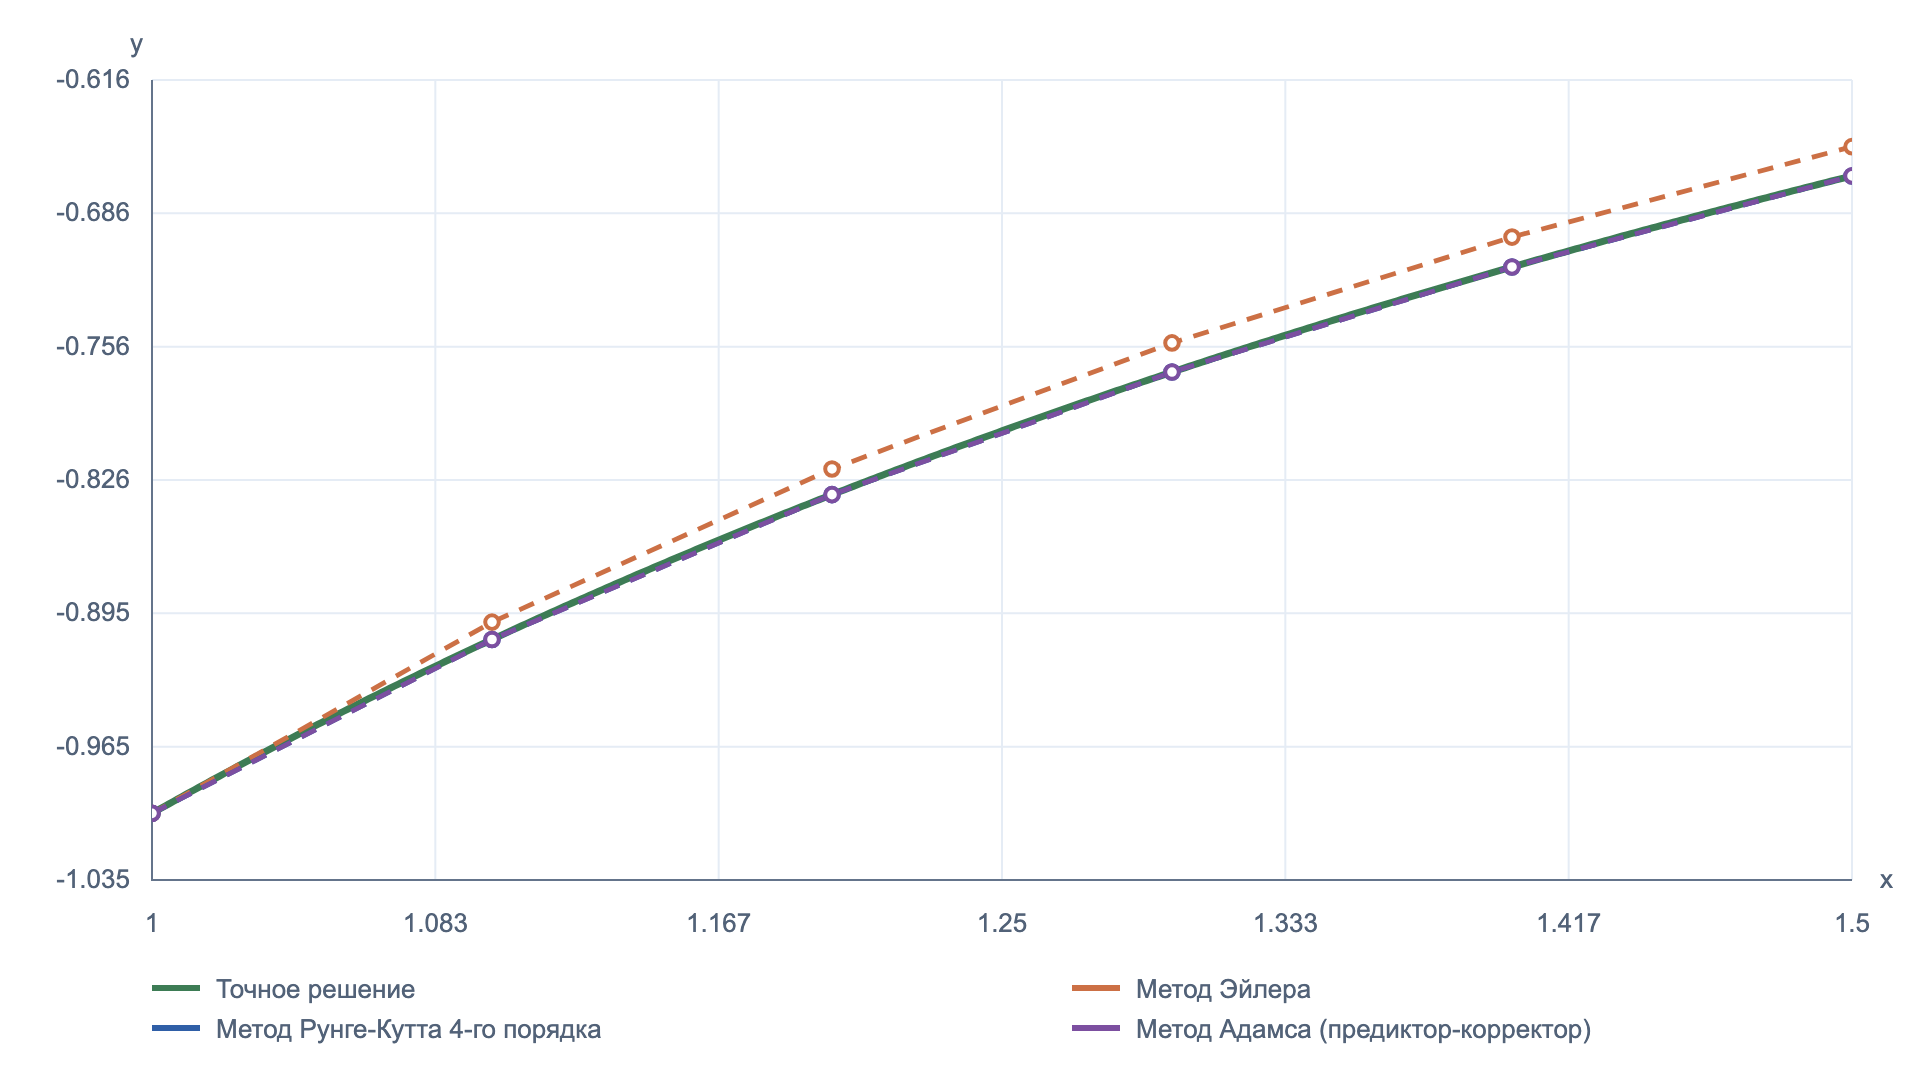
\includegraphics[width=\textwidth]{docs/graph-variant19.png}
\caption{Задача варианта $y'=y+(1+x)y^2$, $y(1)=-1$, $h=0{,}1$:
точное решение (зелёная сплошная линия) и приближённые решения
(пунктир: оранжевый --- Эйлер, синий --- Рунге--Кутта, фиолетовый --- Адамс)}
\end{figure}

Кривые Рунге--Кутта и Адамса визуально сливаются с точным решением,
а ломаная метода Эйлера систематически идёт выше: на каждом шаге приращение
заменяется приращением касательной, поэтому решение «соскальзывает» на
соседнюю интегральную кривую.

\begin{figure}[H]\centering
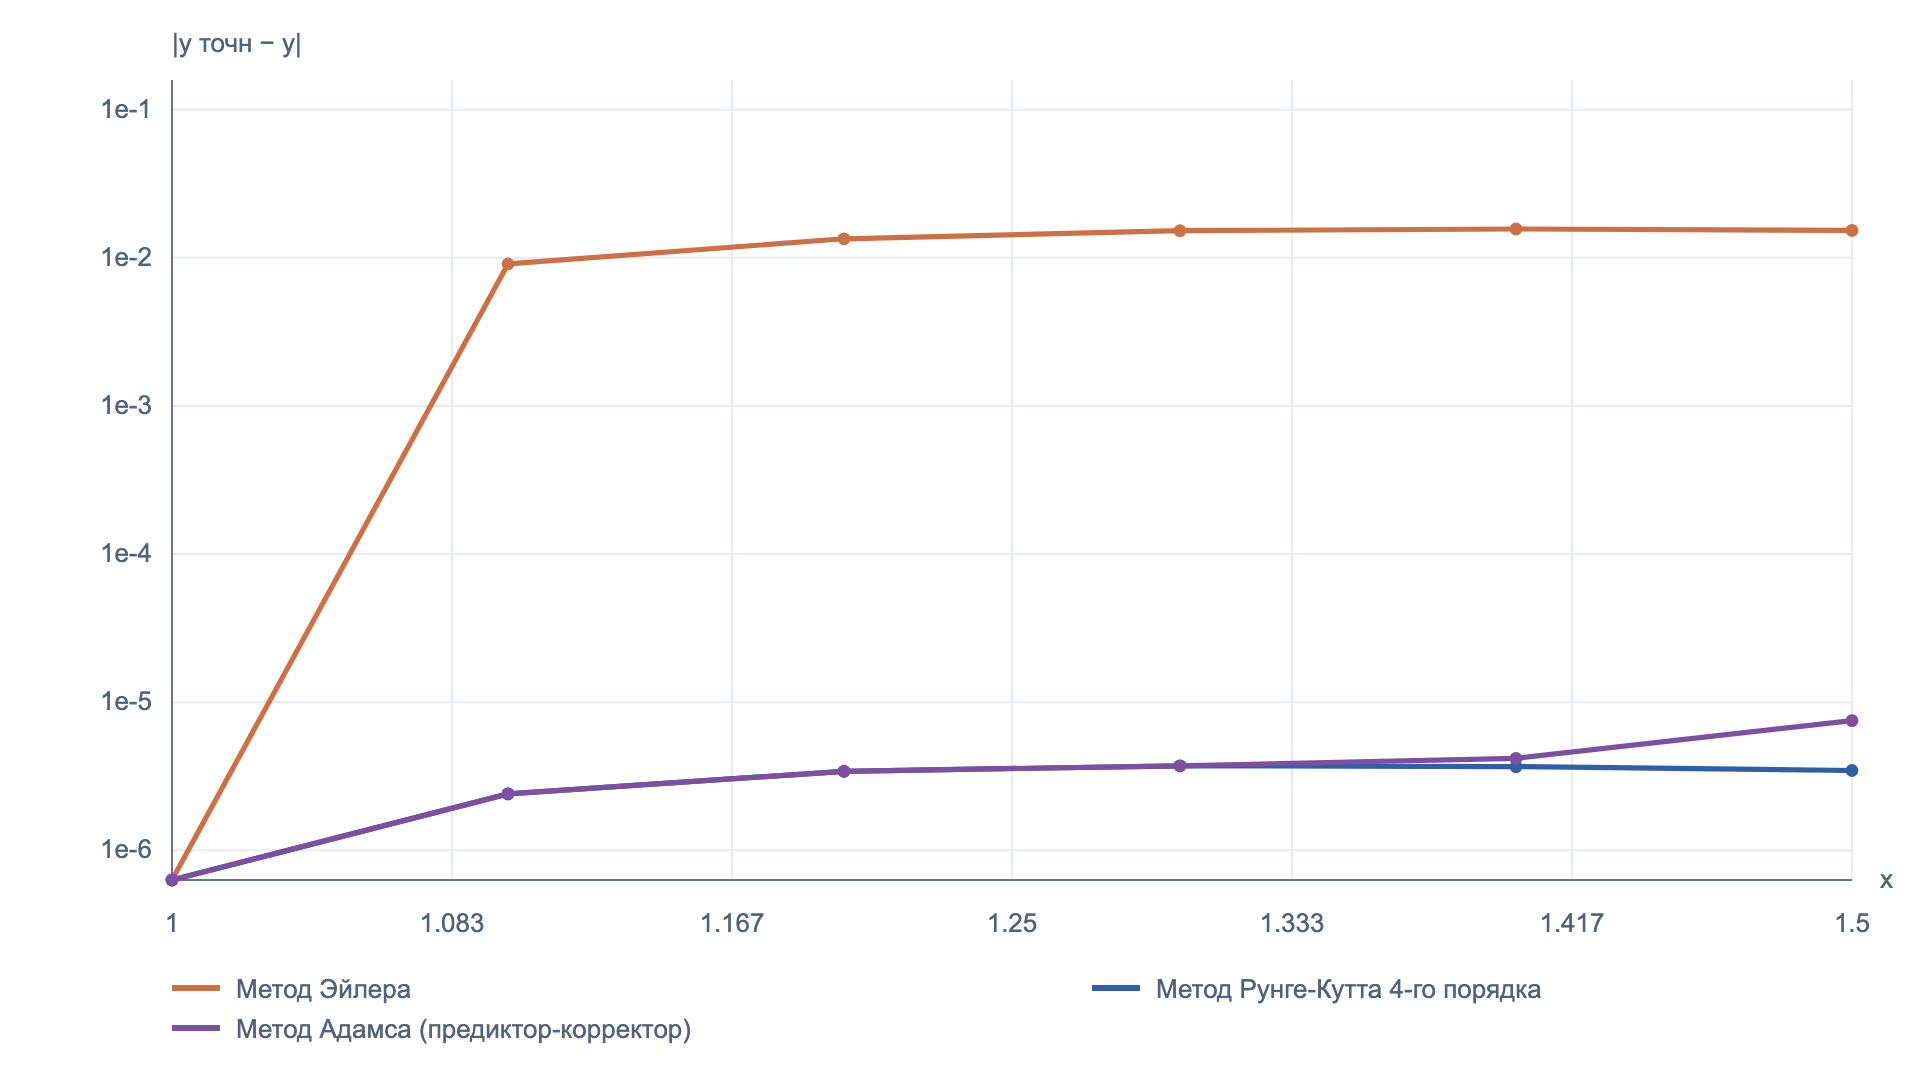
\includegraphics[width=\textwidth]{docs/graph-variant19-error.png}
\caption{Погрешность $|y_{\text{точн}}-y_i|$ в узлах, логарифмическая шкала}
\end{figure}

График погрешности показывает разницу в три-четыре порядка. Видно и то,
что метод Адамса до узла $x=1{,}3$ повторяет метод Рунге--Кутта (эти узлы
получены разгоном), а дальше его собственная погрешность начинает расти
быстрее.

\clearpage
\begin{figure}[H]\centering
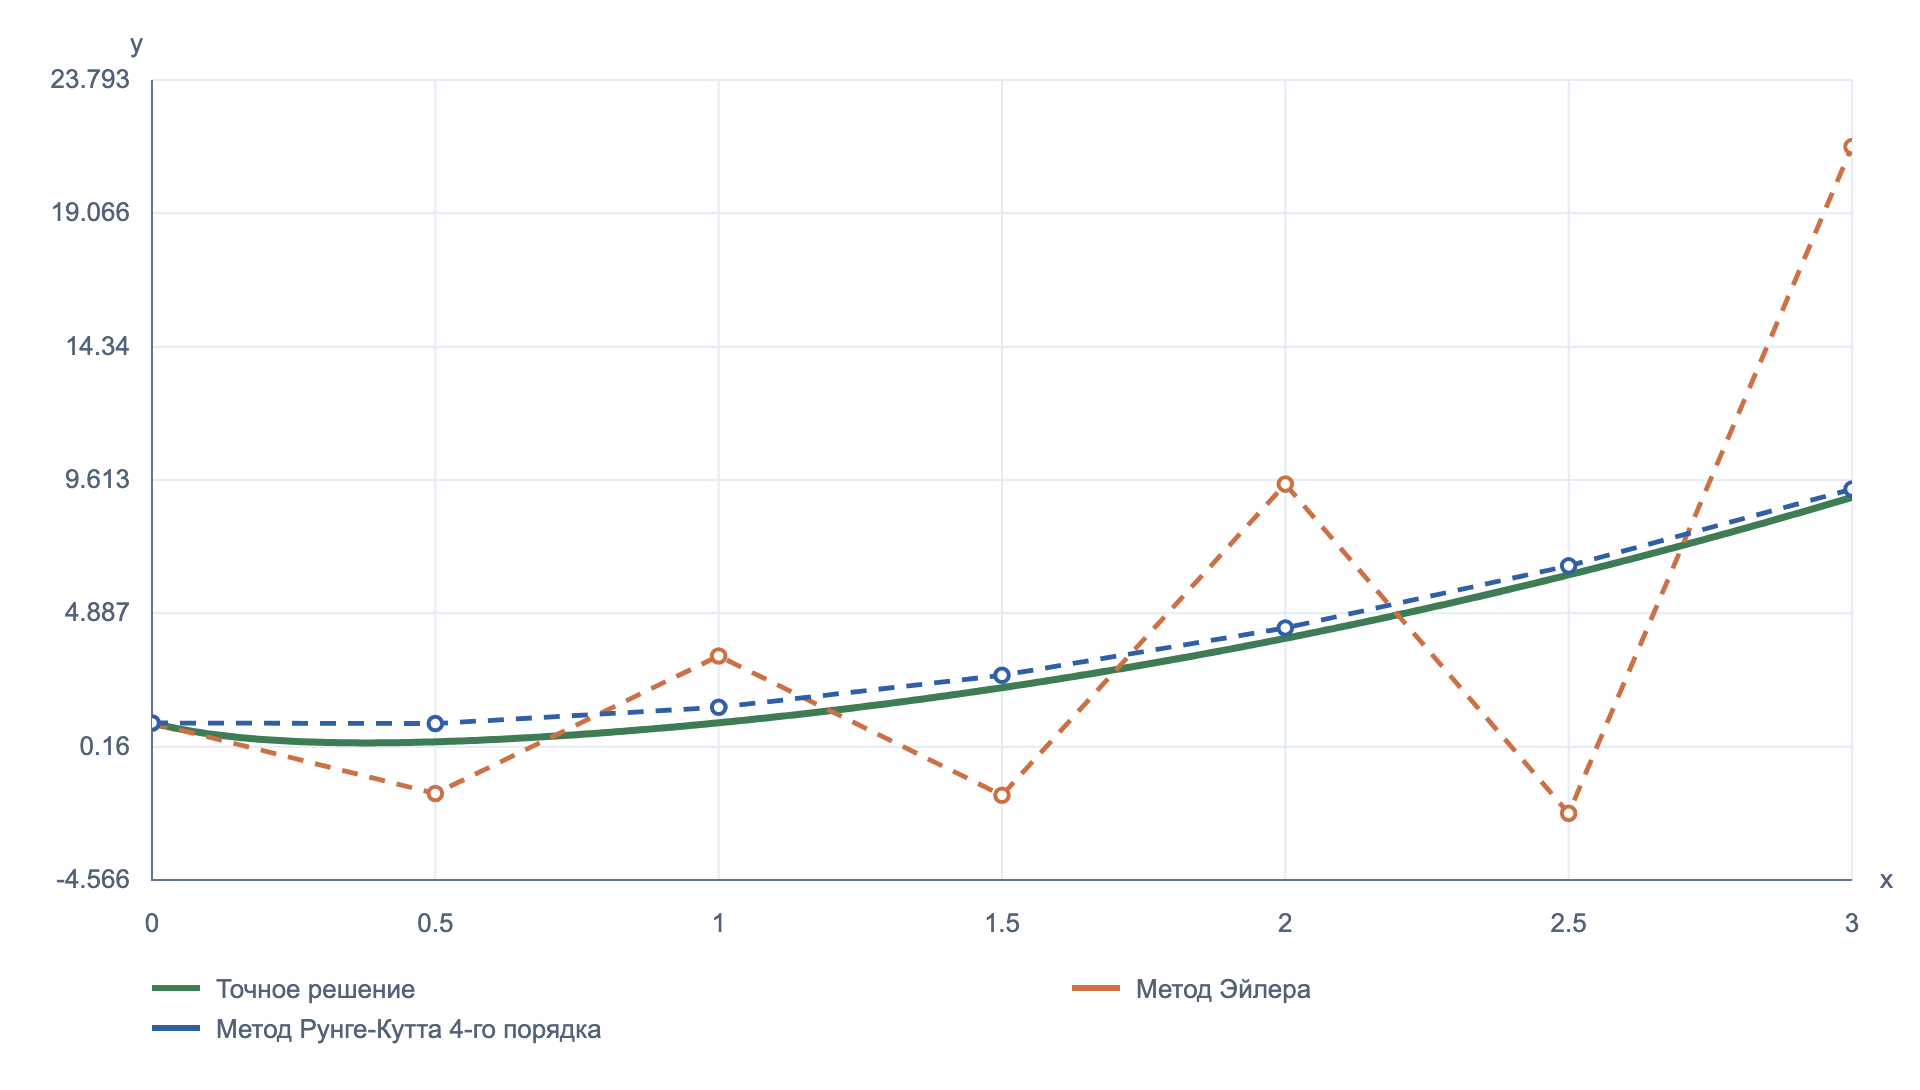
\includegraphics[width=\textwidth]{docs/graph-stiff.png}
\caption{Жёсткая задача $y'=-5y+5x^2+2x$ при $h=0{,}5$: явный метод Эйлера
неустойчив, метод Рунге--Кутта сохраняет качественно верное поведение}
\end{figure}

\begin{figure}[H]\centering
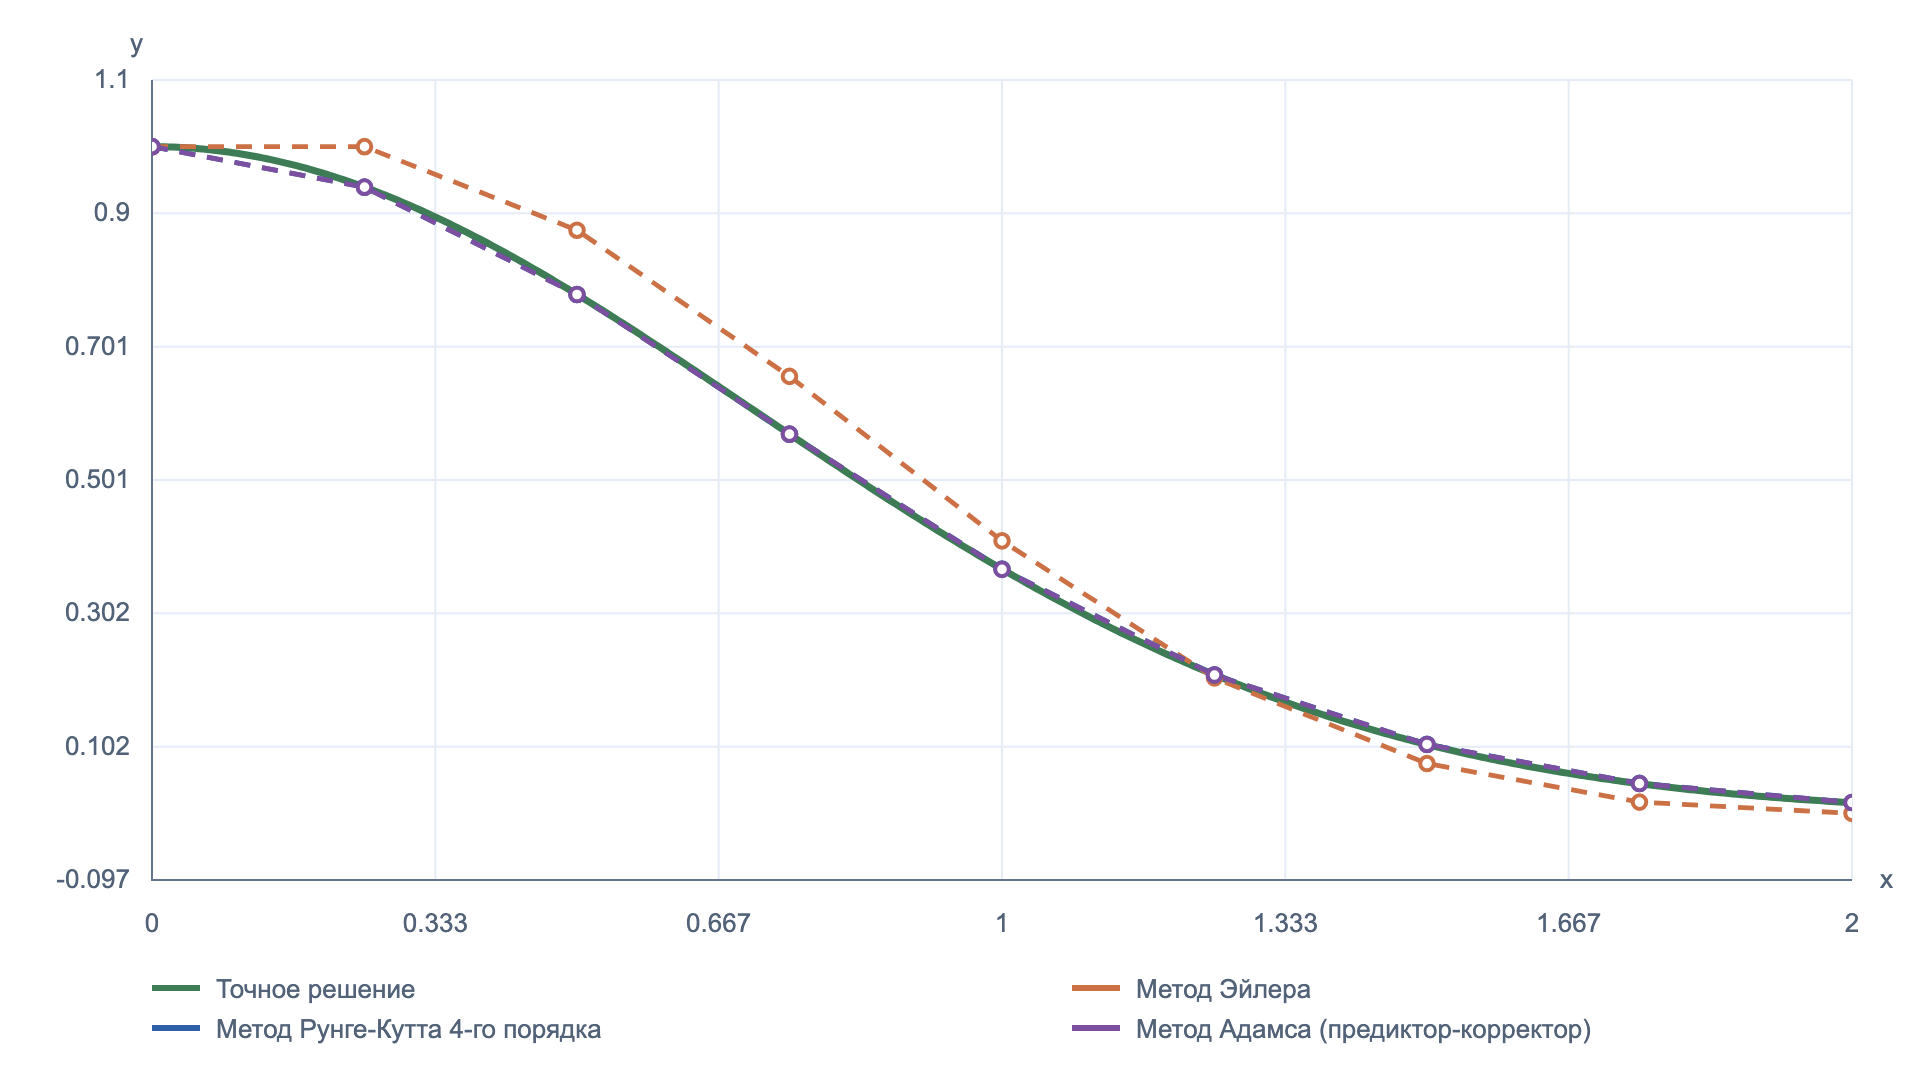
\includegraphics[width=\textwidth]{docs/graph-gaussian.png}
\caption{Уравнение $y'=-2xy$, $y(0)=1$, $h=0{,}25$: крупный шаг заметен
на участке наибольшей кривизны решения}
\end{figure}

% ====================== 7 ======================
\clearpage
\section{Скриншоты результатов работы программы}

Оформление интерфейса продолжает ЛР №4 и ЛР №5: светлый фон, синие акценты,
левая панель ввода и правая область результатов. Ввод $x_0$, $y_0$, $x_n$,
$h$, $\varepsilon$ и выбор уравнения выполняются в одной форме; таблицы,
графики и оценки погрешности обновляются по кнопке «Решить».

\begin{figure}[H]\centering

\includegraphics[width=\textwidth]{docs/screen-web-desktop-report.png}
\caption{Набор 1 --- задача варианта: параметры, сводка по методам и график
точного и приближённых решений}
\end{figure}

\clearpage
\begin{figure}[H]\centering
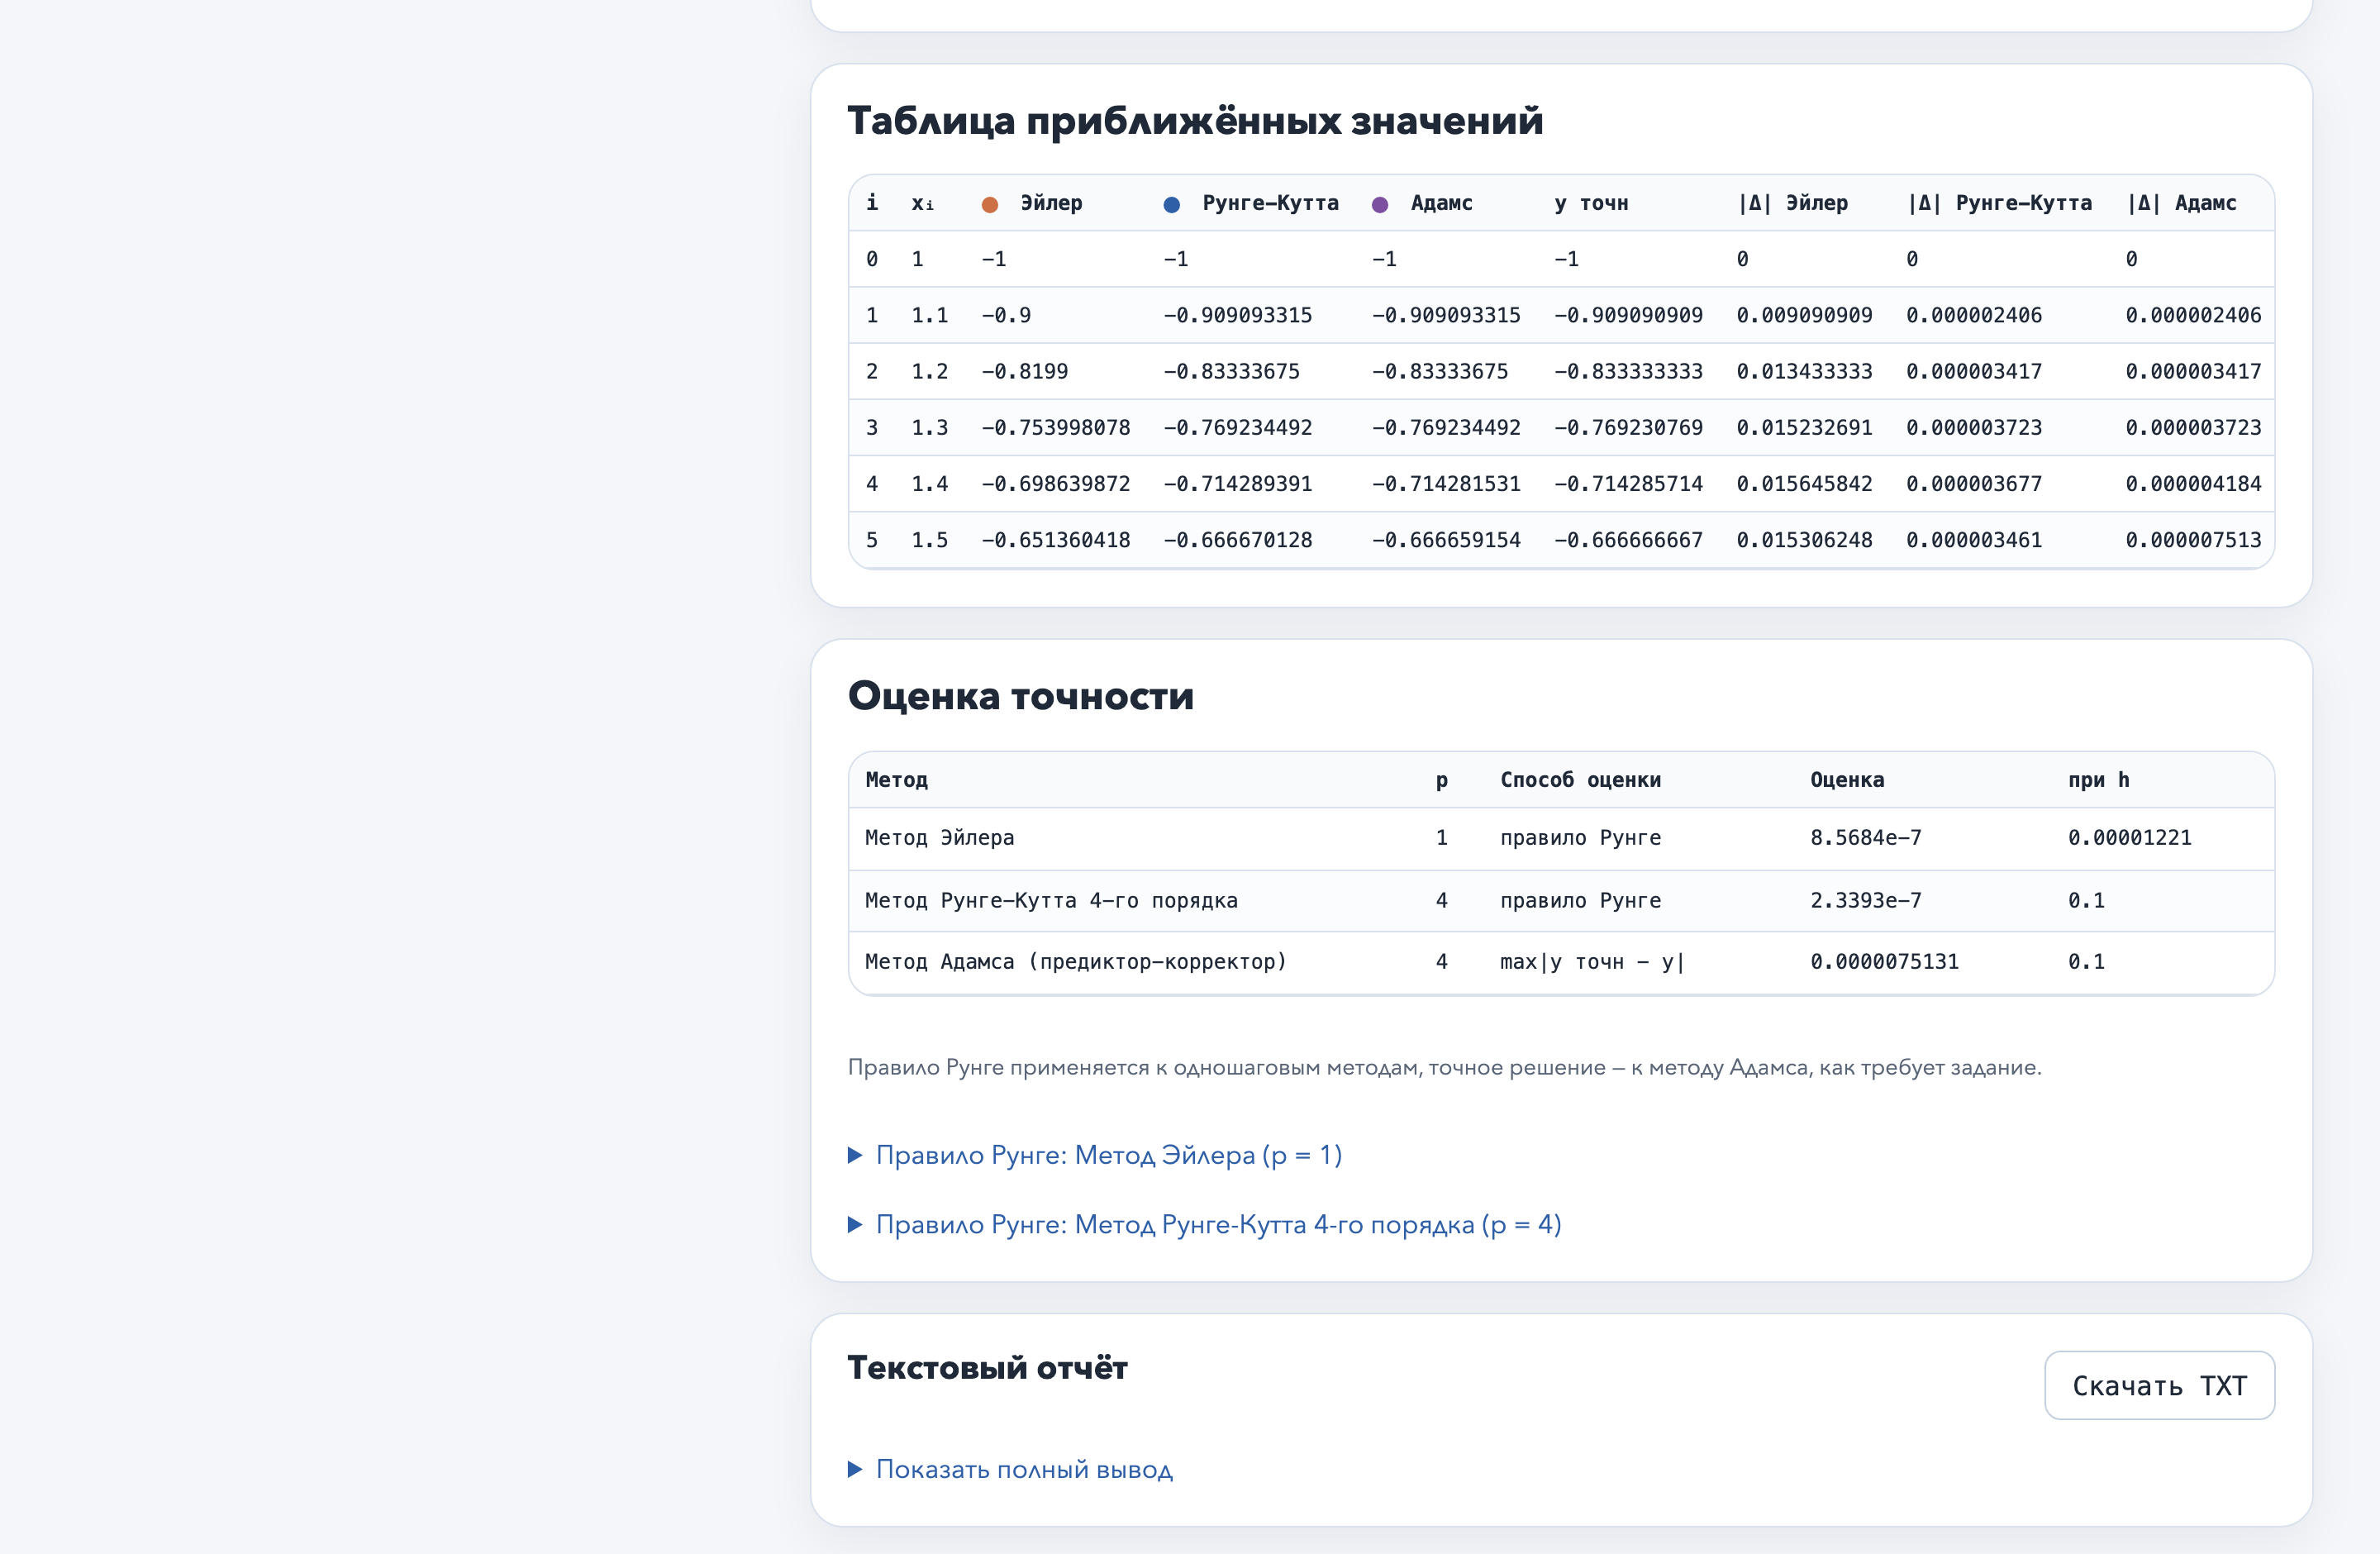
\includegraphics[width=\textwidth]{docs/screen-web-tables-report.png}
\caption{Тот же запуск: таблица приближённых значений с погрешностью в каждом
узле и таблица оценок точности}
\end{figure}

\begin{figure}[H]\centering

\includegraphics[width=\textwidth]{docs/screen-web-stiff-report.png}
\caption{Набор 4 --- жёсткая задача при $h=0{,}5$: предупреждение о большой
погрешности, сообщение о неприменимости метода Адамса и осциллирующая
ломаная Эйлера}
\end{figure}

\clearpage
\begin{figure}[H]\centering

\includegraphics[width=\textwidth]{docs/screen-web-invalid.png}
\caption{Некорректные данные: при $h=-0{,}1$ расчёт не выполняется, выводится
диагностическое сообщение}
\end{figure}

\begin{figure}[H]\centering

\includegraphics[width=0.60\textwidth,height=0.80\textheight,keepaspectratio]{docs/screen-web-mobile-report.png}
\caption{Адаптивная форма в окне шириной 390 пикселей}
\end{figure}

% ====================== РАЗДЕЛ 8 ======================
\section{Вывод}

Решена задача Коши $y'=y+(1+x)y^2$ с начальным условием $y(1)=-1$ на отрезке
$[1;\,1{,}5]$ с шагом $h=0{,}1$ и точностью $\varepsilon=10^{-6}$; точное решение
$y=-1/x$. В точке $x=1{,}5$ метод Эйлера дал $-0{,}651360$, метод Рунге--Кутта
4-го порядка --- $-0{,}666670$, метод Адамса --- $-0{,}666659$ при точном значении
$-0{,}666667$. Погрешность $\max|y_{\text{точн}}-y_i|$ равна $1{,}56\cdot10^{-2}$
у метода Эйлера, $3{,}72\cdot10^{-6}$ у метода Рунге--Кутта и $7{,}51\cdot10^{-6}$
у метода Адамса; значения обоих одношаговых методов совпали с таблицами примеров 1
и 3 лекции.

При $h=0{,}05$ те же погрешности равны $7{,}38\cdot10^{-3}$ и $2{,}15\cdot10^{-7}$,
то есть в 2{,}1 и 17{,}3 раза меньше, чем при $h=0{,}1$. По правилу Рунге точность
$\varepsilon=10^{-6}$ достигнута методом Рунге--Кутта при $h=0{,}1$ (6 узлов),
методом Эйлера --- при $h=1{,}22\cdot10^{-5}$ (40961 узел). Метод Адамса начинает
счёт с $y_4$; значения $y_1$, $y_2$, $y_3$ вычислены методом Рунге--Кутта,
корректор выполняет 3--4 итерации на шаг. Программа выводит сообщение об ошибке
при $h\le0$, $x_n\le x_0$, $\varepsilon$ вне интервала $(0;\,1)$ и нечисловом вводе.

\end{document}
